\documentclass[12pt,oneside,openany,a4paper]{book}
\usepackage{graphicx}
\usepackage[margin=1.4in]{geometry}
\usepackage{lipsum}
\usepackage{enumerate}
\usepackage{enumitem}
\usepackage{indentfirst}
\usepackage[utf8]{inputenc}
\usepackage[hidelinks]{hyperref}
\usepackage[toc,page]{appendix}
\usepackage{xcolor}
\usepackage{listings}
\usepackage{float}
\usepackage{setspace}

\renewcommand{\baselinestretch}{1.15} 

\lstset{
  language=bash,
  basicstyle=\small\sffamily,  
  frame=L,
  columns=fullflexible,
  backgroundcolor=\color{black!10},
  linewidth=0.9\linewidth,
  xleftmargin=0.05\linewidth
}


%----------------------------------------------------------------------------------------
%	TITLE PAGE
%----------------------------------------------------------------------------------------

\newcommand*{\titleGP}{
\begin{titlepage}
\clearpage
\thispagestyle{empty}
\begingroup 
\centering
\rule{\textwidth}{1.6pt}\vspace*{-\baselineskip}\vspace*{2pt} 
\rule{\textwidth}{0.4pt}\\[\baselineskip] 
{\LARGE DEVELOPMENT OF FILTERS FOR\\TRANSCRIPTION BETWEEN\\[0.4\baselineskip] ENGLISH AND BENGALI DOCUMENTS}\\[0.2\baselineskip] 
\rule{\textwidth}{0.4pt}\vspace*{-\baselineskip}\vspace{3.2pt} 
\rule{\textwidth}{1.6pt}\\[\baselineskip]

\scshape 
A Project Report\\
Submitted in Partial Fulfillment of the Requirements\\ 
For the Award of Degree\\
of\\ 
{\large \bf{BACHELOR OF ENGINEERING}}\\ 
\vspace{0.1cm}
\scshape
In\\
{\large \bf{COMPUTER SCIENCE AND TECHNOLOGY}}

\vspace{0.3cm}

By\\[0.2\baselineskip]
{\large \bf{SUSHMITA SEN (Exam Roll-111105027)\\} \& \\ \bf{SURAJEET BHARATI (Exam Roll-111105044)}}\\
[\baselineskip] 

\vspace{0.3cm}

\scshape
Under the Guidance of\\[0.6\baselineskip]
{\large \bf{Prof. MANAS HIRA}}\par 

\begin{center}
				
\includegraphics[scale=0.3]{logo}
\end{center}

{\normalsize DEPARTMENT OF COMPUTER SCIENCE AND TECHNOLOGY\\
\vspace{0.1cm}
INDIAN INSTITUTE OF ENGINEERING SCIENCE\\
AND TECHNOLOGY, SHIBPUR\\
\vspace{0.1cm}
HOWRAH - 711103.\\
\vspace{0.1cm}
MAY 2015}

\par
\endgroup
\end{titlepage}}

%----------------------------------------------------------------------------------------
% DOCUMENT
%----------------------------------------------------------------------------------------
\begin{document}
\pagenumbering{roman}
\begin{spacing}{1.00}
\titleGP
\end{spacing}
%--------------------------------------------------------------
%Certificate
%--------------------------------------------------------------
\thispagestyle{empty}
\begin{center}

\includegraphics[scale=0.2]{logo}\\
\textsc{Department of Computer Science and Technology}\\[0.3cm]
\LARGE{Indian Institute of Engineering Science \& Technology, Shibpur}\\[1.7cm]
\textbf{\emph{\LARGE Certificate}}\\[2cm]
\end{center}

This is to certify that the project entitled, \textbf{``Development of Filters for Transcription Between English and Bengali Documents"} submitted by \textbf{Sushmita Sen} (Exam Roll-111105027) and \textbf{Surajeet Bharati} (Exam Roll-111105044) in fulfillment of the requirements for the award of Bachelor of Engineering in Computer Science \& Technology at the Indian Institute of Engineering Science and Technology, Shibpur,  is an authentic work carried out by them under my supervision and guidance.\\

To the best of my knowledge, the matter embodied in the project has not been submitted to any other University/Institute for the award of any Degree or Diploma.\\[1.6cm]

\begin{flushright}
(Manas Hira)\\
Project Guide
\end{flushright}
\newpage
\begin{center}

%------------------------------------------------------------------
%Acknowledgements
%------------------------------------------------------------------
\section*{Acknowledgments}
\end{center}
\vspace{0.6cm}
\par
\thispagestyle{empty}
After finishing writing the Progress report, it is time now to thank all the people who have helped us through out the process, which makes this thesis possible for us.
\par \vspace{0.2cm}
First of all, we wish to express our sincere gratitude to our guide, Mr. Manas Hira, Professor of the Department of Computer Science and Technology, Indian Institute of Engineering Science and Technology, Shibpur, for providing us such a great opportunity to work with him. We couldn't thank him enough for his knowledgeable guidance, valuable suggestions and continuous encouragement. We are deeply grateful to the efforts, patience and enthusiasm that he shared with us along the entire process. 
\par \vspace{0.2cm}
Many thanks will be paid to all teaching and non-teaching staffs of the Indian Institute of Engineering Science and Technology, Shibpur.
\par \vspace{0.2cm}
We owe to the books, websites and other references wherefrom we have borrowed many of our ideas during project work.
\par \vspace{0.2cm}
Last but not the least, our sincere gratefulness goes to our dearest friends, who were so helpful in every single aspect of our life at Indian Institute of Engineering Science and Technology, Shibpur.

\vspace{6cm}

\hspace{-0.8cm} \rule[0.1cm]{4.8cm}{0.1mm}  \hfill \rule[0.1cm]{4.8cm}{0.1mm} \\
\par \vspace{-0.5cm}
\hspace{0.3cm} Sushmita Sen         \hspace{6.4cm}   Surajeet Bharati \\ 
\par \vspace{-0.5cm}
\hspace{-0.2cm} Date :               \hspace{7.6cm}    Date :   
\par

\tableofcontents
\listoffigures

%-------------------------------------------------------------
%Main Content
%------------------------------------------------------------

\chapter{Introduction}
\pagenumbering{arabic}
In the present scenario of globalization, ethnic populations are no more localized to particular geographic area in the world. There are a lot of people who are not able to stick to their homeland or to some particular place all over his life. Consequently, it is becoming increasingly difficult for such people to remain close to the original culture of the ethnic group to which they belong. For example, it is almost impossible for a Bengali person staying outside the province of West Bengal or the country of Bangladesh to go through a formal schooling for reading or writing Bengali scripts. He or she, therefore, may never have the opportunity to get a direct exposure to Bengali literature. He or she however likely to speak in Bengali when back to his or her own people at his or her residence.If he/she has the Bengali literary works transcribed into some other script or if he/she can transcribe his/her own writing to Bengali script, he or she could have had a glimpses over the Bengali literature.
\par \vspace{0.3cm}
Besides, when most of the concerned people in the present world have at least one smart-phone, tablet or laptop in his hand, they are preferring soft copies more than hard copies for reading purposes. Using hard copies for reading is becoming obsolete day by day. In such cases, they might need some tool to transcribe document into his preferable language script. There comes the importance of having a transcriptor application.

\section{Describing the work}
In the work being proposed, filters are to be designed and implemented for transcription of typed Bengali documents (available in doc, pdf, or HTML formats) into English script and vice-versa. The produced document should be viewable in any web browser and be able to exported to doc or pdf. The transcriptor will be a web application and user will be given the opportunity to transcribe documents using any type of device that has a browser for accessing internet. 

\section{Sectionwise reporting}
This section gives a comprehensive preview of the subsequent chapters of this report. 
\par \vspace{0.3cm}
\autoref{functionalrequirement} describes the functional requirements of the transcriptor that is which services will be provided to the user by the online transcriptor. 
\par \vspace{0.3cm}
\autoref{platform} gives details about the platform that are used to develop and execute the transcriptor.
\par \vspace{0.3cm}
\autoref{design} is concentrated on the details of designing the transcriptor.  Section 1 of the chapter gives the details about the the data-set i.e. data-table used for the purpose of transcription, section 2 gives an insight on the data-structure alternatives that can be used to store our already designed data-set, section 3 will tell you why does a lexical analyzer suite more than some traditional data-structure with respect to our requirements, where section 4 will tell you about different lexical analyzers that can be used.
\par \vspace{0.3cm}
\autoref{implementationpreparation} will give details of the prerequisites needed for starting the implementation. That includes a section about what web server we have chosen among different alternatives and why we have chosen that and other section tell the same about choosing appropriate development tools to reduce the effort.
\par \vspace{0.3cm}
\autoref{implementation} covers the whole implementation process. First section gives broad views about the procedure of transcription between different file formats of different script languages. Second Section includes all the UML design diagrams related to our implementation. In the Third section, you can see web-page interfaces that a user will face while using the transcriptor online and other discussions related to implementation of the front-end.
\par \vspace{0.3cm}
In the last chapter there are three sections which tells about how much of the total requirements we have fulfilled, what we couldn't succeed to implement and what is the future scope of the project one by one. 


\chapter{Functional Requirement}
\label{functionalrequirement}
In this section, we are going to discuss the functional requirements of the online transcriptor that we have developed. A user can get the following services from our developed online tool.
\begin{enumerate}[label=\roman*)]
\item{
As soon as user access the web-page using specified URL, he/she will face a neat and clean interface. In the interface, user will be able to upload a file with extension of HTML, PDF or DOC. He will also be allowed to select the desired output format from a drop down menu which contains three options - HTML,PDF and DOC. User have to tell the system that font of which language he had used in the input file. For this, there will be another drop-down menu containing two options - English and Bengali. Then, clicking on Transcript button will upload the file into server which will be followed by transcription of the input file.
}
\item{
If user selects HTML as output format, then transcribed file will be loaded into user's browser as a normal web-page within a few moments. User can then save the output using \emph{Ctrl+S} or some other key combination depending on the particular browser. For other two output format options, user will get "Download File" prompt in his browser. 
}
\item{
Each word written in Bengali fonts will be converted to equivalent English font while keeping the pronunciation unchanged and vice-versa. The word may be within cell of a table,or it may be a heading, customized text segment or normal body content sentences - each of these have to be transcribed.  
}
\item{
The Transcriptor tool will not transcribe words that are in a image format though, as it works only on objects where \emph{unicode} encoding is there. For working on such images, further image processing algorithms needed and that isn't in our scope.   
}
\item{
One of the main requirement of the online transcriptor is that the look and feel of the input file need to be preserved in the transcribed output file. Only words will be transcribed. All the other things e.g. tables, fonts, font colour, font weight, heading, indentation  etc. will be same as before.
}
\end{enumerate}

\chapter{Platform}
\label{platform}
We have developed the Transcriptor using Java. We have worked on Java version 7.  In this chapter, we will discuss about the platforms used to develop the tool and platforms that have been used to execute our developed system.
\begin{itemize}
\item{We have used Java Servlet for executing our Transcription System on server-side. For this purpose, we have chosen Apache Tomcat(v7.0) web-Server that will be active on server-side to service user requests and transcript documents.}
\item{As mentioned above, the online transcription system has been implemented using Java Servlet.For this we have used Eclipse IDE for EE Developers(Eclipse Luna) to implement the Servlet. Reason behind using Eclipse in our case is that the Tomcat Web-server can be integrated with Eclipse EE IDE.
}
\item{We have used Tomcat Web-server on Ubuntu 14.04 Operating System.}
\end{itemize}
In each of the above mentioned cases, there were several other alternatives that could have been used to get the target achieved. Comparison among them and reason behind choosing a particular one will be discussed on  \autoref{implementationpreparation}.

\chapter{Designing the whole thing}
\label{design}
First of all, we have to design the whole application on the basis of which we can implement the transcriptor. For this case, we have to first design the database.

\section{Designing the Dataset}
For transcription we can use a list containing all the possible words and their transcribed forms. Then we can search for match in the input file and replace it with its transcribed form. This is the approach that all the existing dictionary software use. But this approach is highly inefficient. Storing all such words will take huge memory space and searching word from such a huge list will consume resources and it will be also slow. \par
For speedy transcription of typed Bengali documents to English scripts or vice-versa, we have designed data sets of our own. You can check them in the Figure~\ref{fig:vowel} for Bengali Vowels and digits, Figure~\ref{fig:consonent} for bengali consonants, Figure~\ref{fig:data1}, Figure~\ref{fig:data2}, Figure~\ref{fig:data3} and Figure~\ref{fig:data4} for Benglai Consonant clusters (Juktakkhor).
\begin{figure}
		\caption{Dataset for Bengali vowel}
		\centering
		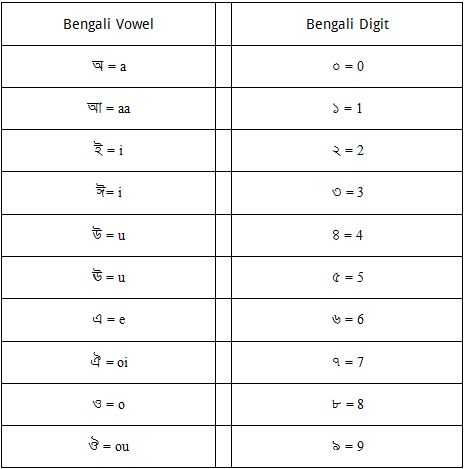
\includegraphics[scale=0.7]{vowel}
		\label{fig:vowel}
\end{figure} \par
\begin{figure}
		\caption{Dataset for Bengali Consonant}
		\centering
		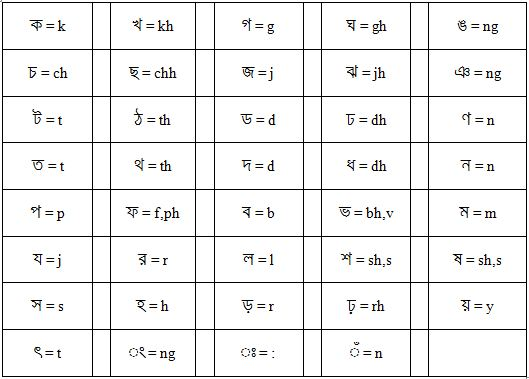
\includegraphics[scale=0.7]{consonent}
		\label{fig:consonent}
\end{figure} \par
Using these dataset, we can easily transcript bengali script to english script as follows.
\begin{center}
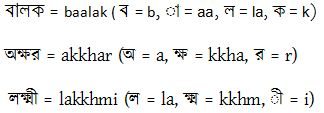
\includegraphics[scale=0.6]{btoe}
\end{center}

That idea will definitely make transcription easier as we have to go through a limited data set during transcription. For transcription mechanism, we need to scan the input file (available in doc, pdf or HTML format)first. During scanning of each character in a word, we will try to get the longest match from the data set for these characters. Then after getting the match according to the data set, we will write the alternate script into the output file. 
\par
In some cases, you can see there are two or more English transcribed form of a single Bengali string in the dataset. Different person can use different English word to write a Bengali word. Such different forms of a Bengali word are listed there. For such English to Bengali transcription, whenever any of these two or more English string will be matched, that will be replaced with the Bengali string. For Bengali to English transcription, whenever the Bengali string is matched, first one among these two or more English strings will be used to replace with.
\par
Now a question can come to your mind that why specifically this data set? Actually the already existing data sets(different standards used by different software) have much more conflicts. So after removing all those conflicts we have come to this one and in future we are going to use this data set as standard. Though it doesn't guarantee that it is completely conflict-free but still we have tried to make it conflict-free as much as possible.  

\begin{figure}
		\caption{Juktakkhor DataSet Table No.1}
		\centering
		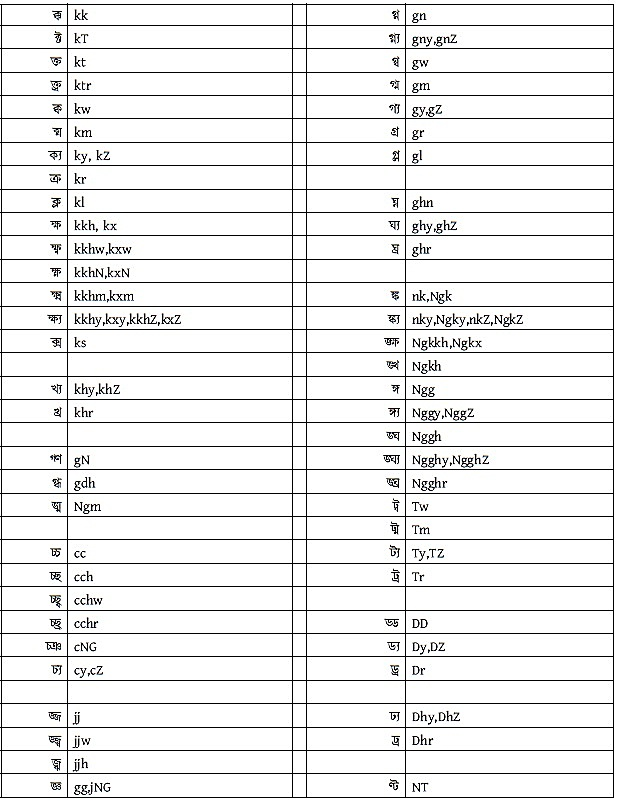
\includegraphics[scale=0.7]{data1}
		\label{fig:data1}
\end{figure}
\begin{figure}
		\caption{Juktakkhor DataSet Table No.2}
		\centering
		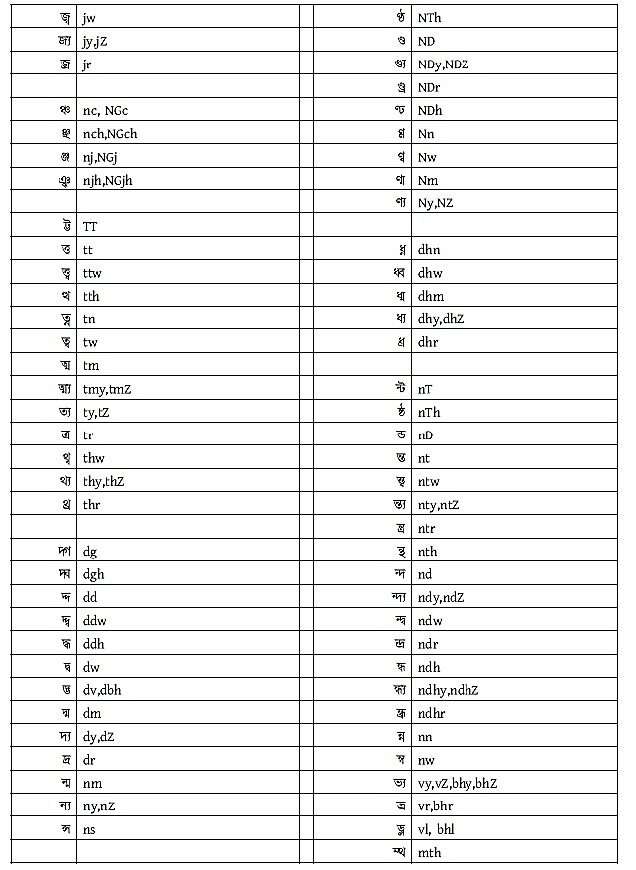
\includegraphics[scale=0.7]{data2}
		\label{fig:data2}
\end{figure}
\begin{figure}
		\caption{Juktakkhor DataSet Table No.3}
		\centering
		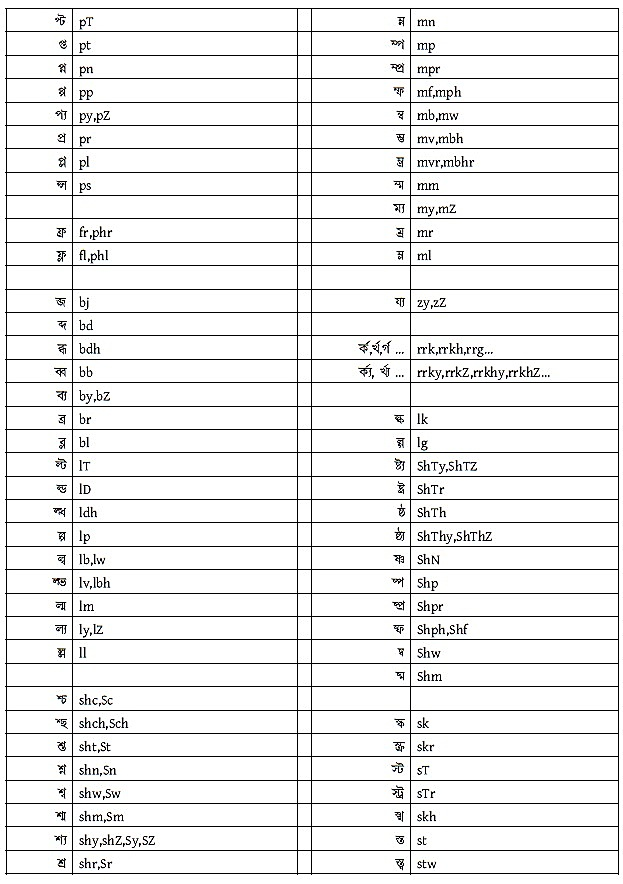
\includegraphics[scale=0.7]{data3}
		\label{fig:data3}
\end{figure}
\begin{figure}
		\caption{Juktakkhor DataSet Table No.4}
		\centering
		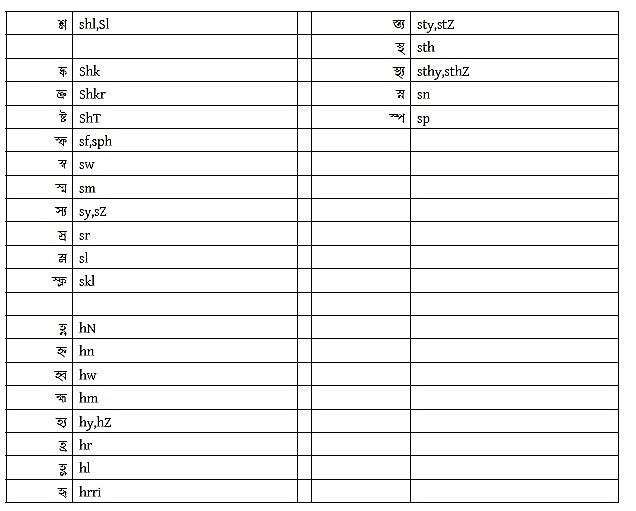
\includegraphics[scale=0.7]{data4}
		\label{fig:data4}
\end{figure}
\par

\section{Datastructure Alternatives}
For storing the data set (as mentioned in the earlier section), we need a proper data structure.  Alternatives for this case are
\begin{itemize}
\item{Dictionary is marked as an obsolete class. So, it should not be used.}
\item{Trie is implemented using tree data structure. It is inefficient in space and time. It should be used when there is an issue of storing a huge dataset with a lot of elements with common prefixes. Our dataset does not follow this characteristic.}
\item{DAWG (Directed Acyclic Word Graph) is used when size of dataset is fixed. Our dataset may be extended dynamically in need.}
\item{HashTable is better when there is a need of multithreading. Possibly, we require single thread in our implementation. So, using hashtable will be just extra overhead. Besides, in hashtable, the hash function has to be implemented by us. So, if we don't implement a good hash function, there will be chance of collision.}
\item{Hashmap supports single thread and good hash functions are already implemented in this class. It’s faster than the other alternatives and suitable for our design goal.}
\end{itemize}
\par
For storing and manipulating groups of objects, hashmap is highly efficient.  Hashmap stores key/value pairs in a hash table. When using a Hashmap, we specify an object that is used as a key, and the value that we want is linked to that key. The key is then hashed, and the resulting hash code is used as the index at which the value is stored within the table. Basically depending upon the matching of longest pattern, we will use this pattern as key and the value will be the alternate script. Here during Bengali to English transcription, key will be Bengali vowel, consonant, digit or complex letters and value will be the English script but for English to Bengali transcription, key will be English pattern and value will be Bengali vowel, consonant, digit or complex letters. As in hashmap, key is hashed and accordingly the value is stored in the table, so we need two different tables for two types of transcription. As using two table will result little bit of space-inefficient (not too much though as our data-set is not such huge), we have tried to implement in such a way that only one table will be in RAM at a time for a particular transcription. For example, during Bengali to English transcription, we will keep that table in memory where key is Bengali pattern and another table will be in disk.

\section{Choosing Lexical Analyzer instead of Datastructure}
Though Hashmap is most suitable among all the alternatives of data structures in case of our design, it will be till an unnecessary use of very heavy thing in comparably smaller issue. It will just result to extra overhead. The data set that we will use for transcription is not so large and Hashmap is not needed to handle it. So, it will be better if we use some lexical analyzer for searching longest match from the input file and replacing it by it's transcribed form instead of using Hashmap datastructure. Some lexical analyzer generator has to be used to generate the analyzer.
\par \vspace{0.3cm}
Using Lexical Analyzer will help us in two significant ways - 
\begin{enumerate}
\item{We don't have to implement any search algorithm or any datastructure for searching purpose. Instead of a lot of lines of Java code, we have to write very easy and small amount lexical analyzer code.}
\item{It implements the analyzer following some fine automata. So, it will be faster in operation than Hashmap datastructure.}
\end{enumerate}

\section{Lexical Analyzer Alternatives}
There are different lexical analyzer generator available that we can use :
\begin{itemize}
\item {Lex is a lexical analyzer generator for generating analyzer in C language.}
\item {JFLex and JLex are most popular lexical analyzer generator for generating analyzer in Java.}
\end{itemize}
As we need to implement the whole design in Java, we can use JFlex or JLex. Between these two JFlex is latest and contains less bug. So, we have used JFlex to accomplish the search and replace function.



\chapter{Preparation for implementation}
\label{implementationpreparation}
\section{Choosing Web Server}
The transcription filter that we are going to implement will run in a Java enabled web server. There are different Java enabled web servers with different sets of functionalities available which are developed by different software development companies. So, firstly we have to choose appropriate web server as per our requirements. Most popular among the web server alternatives are:
		\begin{enumerate}[leftmargin=0.7in]
			\item {Red Hat JBoss (recently renamed to Wildfly)} 
			\item {Oracle Glassfish} 
			\item {IBM WebSphere} 
			\item {Apache Tomcat} 
		\end{enumerate}

	  JBoss, Web Sphere, Glassfish are full stack JavaEE application server that means they include all the JSRs (Java Specification Requests) that are part of a java EE release and whose implementation will be provided by all Java EE certified application servers. On the other hand, Tomcat is just a Java servlet web container. The functionalities, included into the first three are super-set of functionalities included in Apache Tomcat. These three also causes extra resource overhead and administration of these is also complex. So, in case of developing simple web server applications that don't require full Java EE stack, Tomcat can be used. Java EE APIs like EJB or Spring APIs can be imported within Tomcat to extend its functionality. 
\par \vspace{0.3cm}
	Our transcription filter does not require full Java EE stack, it only need native Servlet handling functionalities. There need not be any Security purposes, high resource usage or database transactions. So, we have chosen using Apache TomCat v7.0 with Servlet v3.0.	
	
\section{Choosing Developement tools}
We can use various Java Development Tools (JDT) to simplify the process of developing Java applications (applicable for both Web Application and Standalone java application). They can automate the development process in various ways and decrease the overall effort for developing the application. There are large number of JDTs, available for almost all stages of software development. Some of the mostly used JDTs are mentioned here.
\begin{itemize}
\item	Integrated Development Environments (IDEs) like Eclipse, NetBeans, Boreland Together, BlueJ are added with various debugging tools and convenient functions that make writing the program and debugging much easier than using command line. We will use Eclipse 4.4 Luna to implement the filter.
\item	We can use automation tools like Apache Ant or Apache Maven to automate various processes like building, compiling, restarting server etc.
\item	Documentation creating tools like javadoc can be used to create documentation of our implementation. 
\item  Using Java Mission Control we can control running Java programs and resources used by them.
\item Apache Torque is an object-relational mapper using which database script can be generated and executed automatically to control a database. It provides high level of abstraction and hides all database-specific implementation details.
\end{itemize}

Initially we will start using Eclipse 4.4. It can detect unused or unreached code segments or variables in source codes, build source codes to some specified location. Apache Tomcat 7.0, which we are going to use as web server, can also be integrated with Eclipse. In future, we can use other development tools if required.



\chapter{Implementation}
\label{implementation}

\section{Transcription between different formats}
Till now, the online tool can provide the facility to transcript a Bengali script of HTML or PDF format into a English script of HTML, PDF or DOC format and a English script of HTML or PDF format into a Bengali script of HTML, PDF or DOC format. The procedure of those transcription are discussed below.
\subsection{HTML to HTML}
In case of HTML to HTML transform, when we transcribing from Bengali document to English Document, we only search for Bengali longest match (in unicode encoding) in the data-set and replace them with corresponding English form. So, all the HTML tags or HTML related words will be unaffected. That will result to a output file, look and feel of which will be same as input file where Bengali words will be transcribed to English words.

When we are transcribing a English document to a Bengali document, we will exclude all those words which are between HTML tags i.e. between ``$<$" and ``$>$"  and search for longest match in the rest to replace it with its Bengali form.

\subsection{HTML to PDF}
In both cases of Bengali to English transcription and English to Bengali transcription, at first input file will be converted to transcribed HTML file in the procedure that are mentioned in above subsection. Then that output HTML file will be converted to PDF format.

Now for this format conversion, we have to remember one thing : we have to preserve the look and feel of the input file after transcription. But, all best open source Java API e.g. \emph{PDFBox}, \emph{iText} etc failed to fulfill this requirement.

Now, we have solved that issue using \emph{wkhtmltopdf}. It uses Web Kit Renderer, the same rendering engine that is used by Google Chrome or Apple Safari to render a HTML page. But the only problem was that this renderer is implemented using C and they does not provide any Java API. This problem remains same for another renderer namely Gecko (used by Mozilla Firefox). \emph{wkhtmltopdf} provides a command line tool to convert HTML document to a PDF document without changing the look. We installed that tool on our Ubuntu Machine and created new Process of \emph{wkhtmltopdf} from our servlet to convert HTML to PDF. This process is using much low RAM space ($<$1MB), low CPU for creating a PDF and also terminating within a moment every time. So, we think, it will be acceptable to be run on server. The output PDF has exactly same look as the input HTML document. 

Some commercial Java API like \emph{NitroPDF}, \emph{PDFCrowd} might be useful though. In fact converted document examples in PDFCrowd Website looks quite promising. We haven't tested those API as we are only dealing with open source API.

\subsection{HTML to DOC}
In this case, input file will be transcribed into a PDF file following above-said procedure. Then the the PDF will be converted to DOC file. For this conversion, we have used \emph{Apache PdfBox}.

\subsection{PDF to Other Formats}
We faced several problems when working on this transcription. Here, the problem is again conserving the look and feel of the input document. We can transcribe the PDF document by using three different procedures as follows, 

\begin{enumerate}[label=\roman*)]
\item{We can extract texts from the PDF file using \emph{PDFBox} Java API and then transcribe those text using parser and then converting those transcribed text to a file of any format that user want. But, the problem is when we are extracting the text from PDF, we are losing everything about the look of the PDF (some part like indentation, margin remains same though). So, one of our objective failed. It is quite impossible to carry information about look of the PDF while extracting the text, as a PDF file have its own objects, reference table, different level of abstraction that are hard to manage through programming. So, we left this idea and started thinking some other ways to fulfill our objective.}
\item{The second method that we thought is parsing the PDF file, extracting each word, and replacing the word with its transcribed form. In that case, we do not have to think about the look and feel of the PDF, as we are just replacing the string in the PDF without effecting all the other information. Real challenge here is replacing a word in a PDF file. Though all the APIs like \emph{PDFBox}, \emph{iText}, \emph{PDFLib} demand that they can do it, but they failed in 95 percent cases. After a round of net surfing, we discovered that replacing a word in PDF is also quite complicated task and any type of implementation will fail in maximum cases. We haven't tried any commercial APIs like \emph{AsposePDF} though. May be, they will work well in the case of replacing a word or converting to other format.}
\item{Another thought was converting the PDF to equivalent HTML and then work on the HTML. We got a Java API namely \emph{PDF2DOM} for this purpose. But, it failed to render a PDF file to similar HTML file correctly. In the output HTML file, consecutive strings are overlapping on each other making the whole document illegible. There is a Commercial API namely \emph{JPEDAL}, which we haven't tried yet.}
\end{enumerate}

So we ultimately decided to just extract text from the PDF and transcribe those text to get atleast the transcribed text from the input file. In this way, the look and feel of the input PDF document got completely lost. 

\subsection{DOC to Other Formats}
After those work with PDF file, we started working with DOC format, and discovered that internal structure of a DOC file is messier than the PDF file. Sometimes, it differ in its internal structure just because of difference between the Office tools used to write the DOC file. So, even extraction of text from a DOC document fails sometime.

There are some Java API like \emph{Apache POI}, which are used to handle DOC file, replace word in a DOC file, or extract words from a DOC file. But, it is only usable for DOC created by Microsoft Office. We haven't tested this API though.

\section{UML Diagrams}
\subsection{Use Case Diagram}
\begin{figure}[H]
		\caption{Use case Diagram}
		\centering
		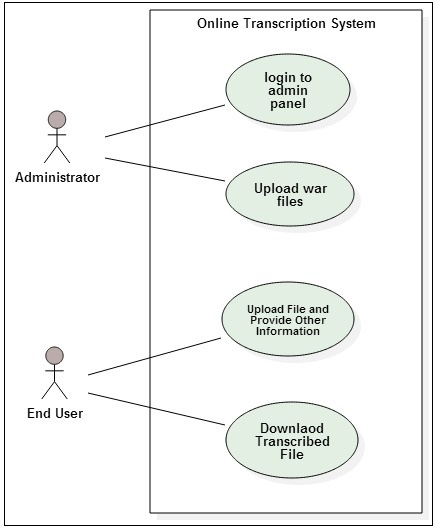
\includegraphics[scale=1.1]{usecase}
		\label{fig:usecasediagram}
\end{figure} 

\subsection{Class Diagram}
\begin{figure}[H]
		\caption{Class Diagram}
		\centering
		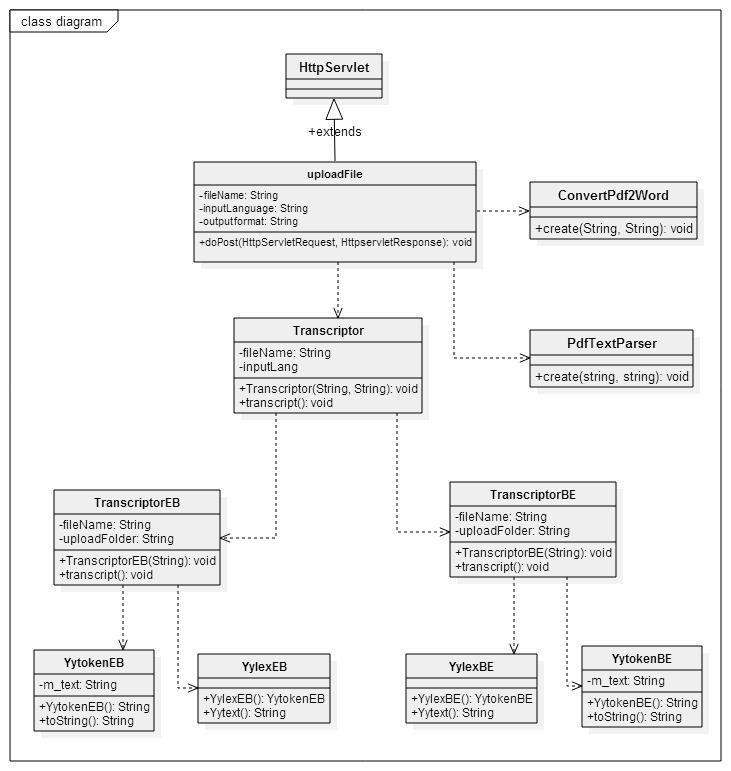
\includegraphics[scale=0.58]{class}
		\label{fig:classdiagram}
\end{figure} 

\subsection{Sequence Diagram}
\begin{figure}[H]
		\caption{Sequence Diagram}
		\centering
		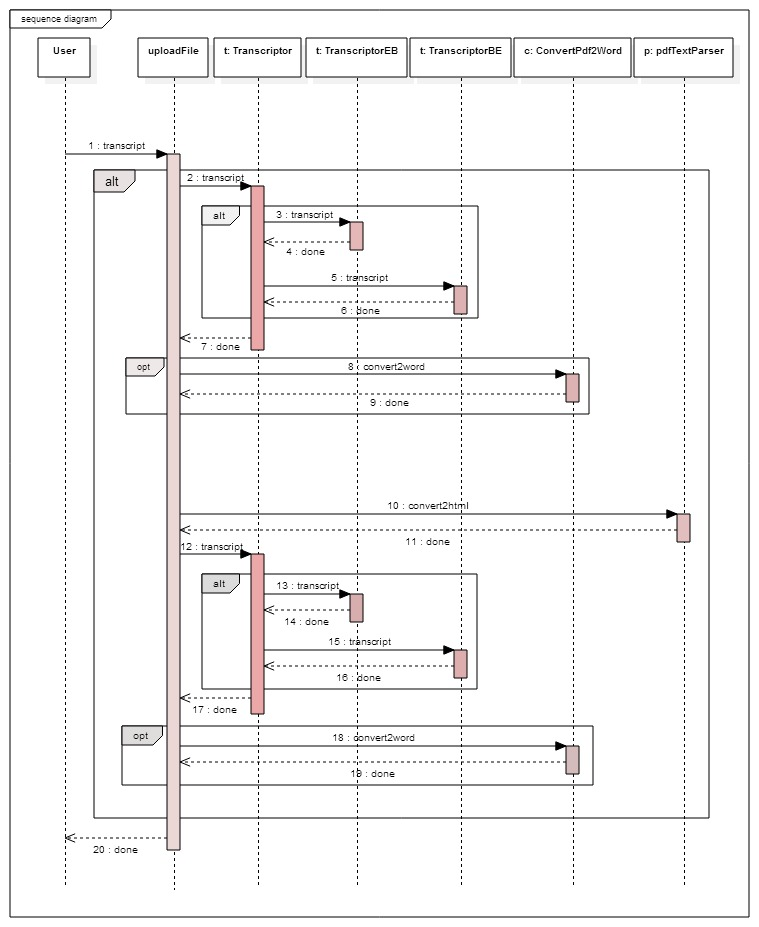
\includegraphics[scale=0.56]{sequence}
		\label{fig:sequencediagram}
\end{figure} 

\section{Designing the GUI}
As said before, our transcriptor will be a web application that will run on server-side and user can access it and transcribe his document using a website and corresponding web-pages. 
\subsection{Programming Languages Used}
The web-pages should be neat and clean, easily understandable, interactive and easily usable. To design the web-pages we have used the following languages:
\begin{itemize}
\item {HTML: We have used HTML5 to develop the skeleton of the web-pages. Using HTML, we have designed file upload button, drop down list, or the submit buttons}
\item {CSS: We have used CSS3 to describe the presentation of Web pages, including colors, layout, and fonts. It has made the web-pages more sophisticated by controlling the look and feel.}
\end{itemize}

\subsection{Designed Webpages}
We have designed only one page as per the requirement. That is the home page that will be faced by the user at the very first. This page can be accessed through \emph{http://purity.becs.ac.in:8080/test-app/}. Take a look on Figure ~\ref{fig:homepage}. It is the home page. In order to transcribe a file, you have to upload the file using "Browse File" button. Then you have to choose your desired output format (HTML, PDF, DOC) from the drop-down menu and have to also tell font of what language used in the input file (English or Bengali). Then you can transcribe the file. If you have chosen the output format as HTML then the output will be shown as an web page that you can save. Otherwise the output will be downloaded.
\par \vspace{0.3cm}
Here, you can see, you need not to provide the input format and whether it is Bengali script or English script. This information will be detected internally. 
\par \vspace{0.3cm} 
\begin{figure}[H]
		\caption{Home Page Design}
		\centering
		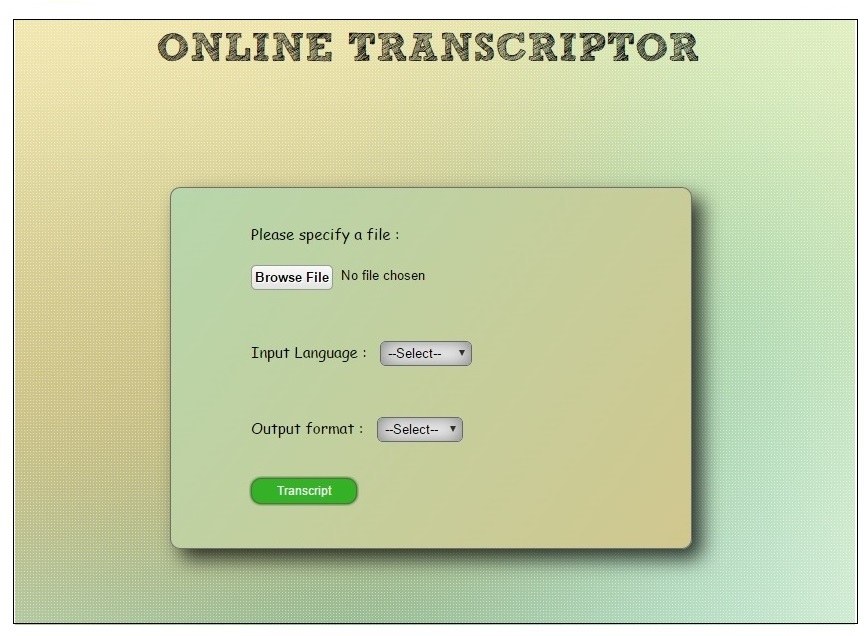
\includegraphics[scale=0.6]{interface}
		\label{fig:homepage}
\end{figure}
\par





\chapter{Conclusion and Future Scope}
\label{conclusion}
\section{What we have done}
We have completed the whole project and tried to reach all of the requirements as much as possible. We are briefly mentioning what portions of the requirements are completed.
\begin{enumerate}[label=\roman*)]
\item{We have completed whole of the design phase. We have designed the whole data-set using which transcription have been done. This data-set have been used as standard for the implementation till the end. We have tried to make the data-set free of conflicts as much as possible. Those data-sets have been shown before.}
\item{We have chosen appropriate one among various alternative to store this data-set and searching it in a highly efficient way. That have maximized the speed of the process of transcribing a document.}
\item{We have chosen java servlet enabled web server and java development tools as per our need so that we can implement the design without any interruption.}
\item{We have successfully designed and implemented transcriptor for transcribing typed Bengali documents available in HTML format into English script (exportable to HTML,DOC and PDF format) and vice-versa. But in conversion from PDF to HTML we are losing the look and feel and so in the case of PDF to other formats. In case of DOC format, we are facing the same problem. Ignoring the look and feel,we can successfully transcript the script in any format which is of bit more importance than keeping the look and feel. UNICODE Encoding and JFlex Parser are working well to manage this conversion.}
\item{We have designed the front page of the website through which user will interact with the online transcriptor. We have tried to make the page easily usable and good to look at.}
\end{enumerate}

\vspace{0.5cm}
\par

\section{Limitation in the design and implementation}
We have tried to reach all of the requirements as much as possible. But, still, some part of the requirements seemed impossible or something between extremely hard and impossible. There are some important issues or better to be said as problems that are worth mentionable here as till now we think those problems cannot be solved in our proposed designed approach.

\subsection{Limitation in data-set}
Though we have completed designing the data-set, but it is not completely free of conflicts. We have tried to find and remove those conflicts as much as possible but removing all of those is not possible actually.

Reason of those conflict are some language specific pronunciation anomalies.As a result, some words will be transcribed to some unexpected form. Example of some of such English words are BUS, DO, GATE etc. The transcribed form of such words will loose the original pronunciation. Even if we try to remove this problem as much as possible, it is not possible to remove all such problems with respect to our design approach.

\subsection{During File Format Conversion}
The look and feel of the transcribed document is not same as the original document. For the case of HTML to HTML and PDF conversion, we are successful to make the transcribed form of the document absolutely same as original document but for other cases, it is very hard to make the look same.

From PDF to HTML conversion,we are losing the look and feel of the source or original document. Actually, PDF documents are not supposed to be word-processed. They are designed completely considering the idea of portability so that irrespective of hardware architecture or operating system, a PDF file gives same representation when opened. For this, it internally uses its own data types,data structures,objects,reference table and separate levels of abstraction,design of which also differ from PDF version to version.So, it is very hard to process a PDF file programmatically. 

We faced same problem with DOC format, and discovered that internal structure of a doc file is messier than pdf file.Sometimes it differ in its internal structure just because of difference between the office tools used to write doc file, So, even extraction of text from a doc fails sometimes.

\vspace{1cm}


\section{Future Scope}

In this section we can discuss how the quality of the transcriptor can be improved by extending the existing design approach that is made by us and already discussed. 

The limitation in data-set that is discussed in last section can be resolved by integrating a list of such common words. Input file will be parsed for searching those words and replacing them with their correct transcribed form that are also available in the same list. Other words will be dealt as usual. Though this brute force approach will be highly inefficient, but it will decrease the rate of such errors when as well as decreasing the speed of the process of transcription. 

To resolve the issues regarding file format conversion, some commercial Java API can be bought and tried though they may also fail. 

\vspace{0.3cm}
Our designed transcriptor can be extended to some more sophisticated form. There are many people who can speak in a language but can't write in that language. Using our design approach some tool can be made for them in future such that they can write words of that language in alphabet of a language that is known to him and then converting that written document to that other language script.

\vspace{2cm}
\begin{center}
\rule[3cm]{2cm}{0.1mm}
\end{center}


\begin{appendices}


\chapter{Installation and User Manual}

In this chapter, we have briefly discussed the installation procedure of the online transcriptor system that we have developed.

Firstly, \emph{tomcat7} server have to be installed and configured in a computer where \emph{ubuntu} OS is used following the steps discussed below.

\begin{enumerate}[label=\roman*)]
\item{First of all, \emph{tomcat7} server have to be installed. That can be done on a \emph{ubuntu}  machine using the following terminal commands. 
\begin{lstlisting}
   sudo apt-get update
   sudo apt-get install tomcat7
\end{lstlisting}
This command will automatically install \emph{openjdk7}, if it is not already installed as \emph{tomcat7} need \emph{Java} to operate. }
\item{\emph{tomcat7-admin} have to be installed to be able to upload \emph{war} files remotely into the \emph{tomcat server}. To install \emph{tomcat7-admin}, one can use following command.
\begin{lstlisting}
   sudo apt-get install tomcat7-admin
\end{lstlisting}
}
\item{
To work with \emph{tomcat7-admin}, it have to be configured firstly. A login have to be added to the \emph{tomcat} server. This can be done by editing the \emph{tomcat-users.xml} file as follows.
\begin{lstlisting}
   sudo gedit /etc/tomcat7/tomcat-users.xml
\end{lstlisting}
This file is filled with comments which describe how to configure the file. You may want to delete all the comments between the following two lines, or you may leave them if you want to reference the examples:
\begin{lstlisting}
   <tomcat-users>
   </tomcat-users>
\end{lstlisting}
You will want to add a user who can access the \emph{manager-gui} and \emph{admin-gui} (the management interface that we installed in Step Two). You can do so by defining a user similar to the example below. Be sure to change the password and username if you wish:
\begin{lstlisting}
   <tomcat-users>
       <user username="admin" password="password" 
         roles="manager-gui,admin-gui"/>
   </tomcat-users>
\end{lstlisting}
Then the \emph{tomcat-users.xml} file have to be saved and quit.
}

\item{Next, we have to start \emph{tomcat7} service to work with it. We can use following command
\begin{lstlisting}
   sudo service tomcat7 start
\end{lstlisting} 
We can stop or restart \emph{tomcat7} when needed using following two commands respectively.
\begin{lstlisting}
   sudo service tomcat7 stop
   sudo service tomcat7 restart
\end{lstlisting}
}
\item{
After starting \emph{tomcat7} service, we have to upload the \emph{war} file that is provided with the source code DVD. For this purpose, we have to open the admin-panel.We can access admin panel using the following url 
\begin{lstlisting}
   http://your_ip_address:port/manager/html
\end{lstlisting}
You will be asked to enter \emph{username} and \emph{password}. Once you give it correctly, you will be redirected to admin panel. In the admin panel, you will get button to upload and deploy \emph{war} file.
}
\item{
After deploying the \emph{war} file, your can access the online transcriptor. If the \emph{war} file name is \emph{test-app.war}, then you can access the system using the following url 
\begin{lstlisting}
   http://your_ip_address:port/test-app
\end{lstlisting}
}
\item{You can change source code when needed using some IDE, create new \emph{war} file and deploy the \emph{war} file in the \emph{admin-panel} to get the changed behavior.}

\end{enumerate}

\chapter{References}
\begin{enumerate}
\item{Head First Java by \emph{Bert Bates and Kathy Sierra}}
\item{Java The Complete Reference - 8th Edition by \emph{Herbert Schildt}}
\item{Head First Servlets and JSP by \emph{Bert Bates and Kathy Sierra}}
\item{Java Servlet Programming, 2nd Edition by \emph{Jason Hunter, William Crawford}}
\item{lex \& yacc, 2nd Edition by \emph{Doug Brown, John Levine, Tony Mason}}
\item{www.coreservlets.com}
\item{https://tomcat.apache.org/}
\item{www.stackoverflow.com}
\item{www.wkhtmltopdf.org}
\item{www.eclipse.org}
\item{http://jflex.de/manual.html}
\end{enumerate}

\chapter{Source Code(DVD)}

\end{appendices}

\end{document}
